\chapter{Interference}

\section{Preposition}

Two beam of light may interfere when:

\begin{itemize}
\item not perpendicular
\item has same frequency
\item has stable phase shift
\end{itemize}

\section{Algorithms}

Two wave of light $\vec{E}_1$ and $\vec{E}_2$

\begin{equation*}
  \begin{aligned}
    \vec{E}_1 = \vec{\varepsilon}_1 \exp \left[ i \left( \vec{k}_1 \cdot \vec{r} - \omega_1 t + \delta_1 \right) \right] \\
    \vec{E}_2 = \vec{\varepsilon}_2 \exp \left[ i \left( \vec{k}_2 \cdot \vec{r} - \omega_2 t + \delta_2 \right) \right]
  \end{aligned}
  \quad \Rightarrow \quad 
  \begin{aligned}
    I &= \left< \left| \left( \vec{E}_1 + \vec{E}_2 \right)^2 \right| \right> = \varepsilon_1^2 + \varepsilon_2^2 + 2 \vec{\varepsilon}_1 \cdot \vec{\varepsilon}_2 \cos \varphi \\
    \varphi &= \left( \vec{k}_2 \cdot r - \vec{k}_1 \cdot r \right) + \left( \omega_1 - \omega_2 \right) t + \left( \delta_2 - \delta_1 \right)
  \end{aligned}
\end{equation*}

\section{Young's Experiment}

\begin{figure}[H]
  \centering
  \begin{subfigure}{.55\textwidth}
    \centering
    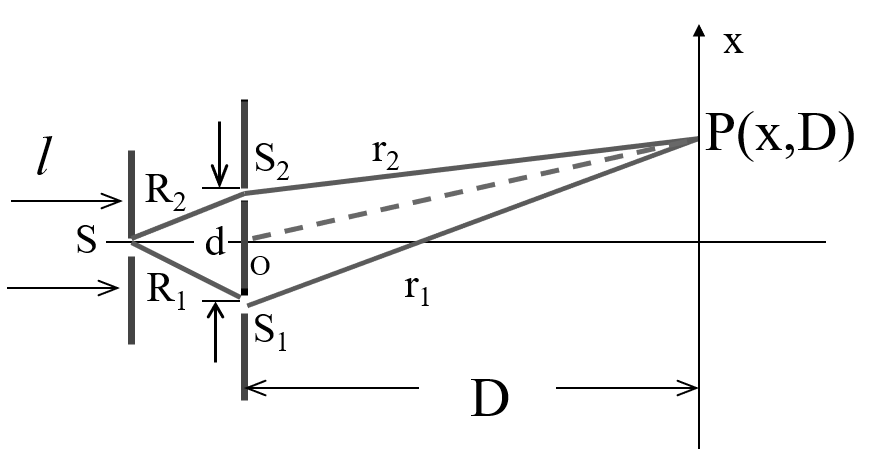
\includegraphics[width=\linewidth]{figures/Young-Exp}
  \end{subfigure}
  \begin{subfigure}{.35\textwidth}
    \centering
    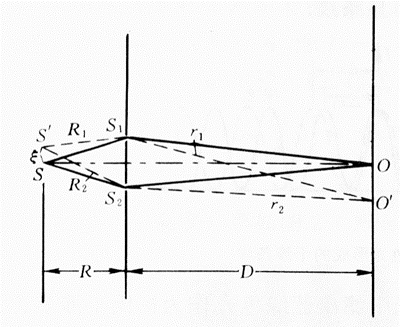
\includegraphics[width=\linewidth]{figures/Young-Exp-2}
  \end{subfigure}
\end{figure}

\begin{equation*}
  \begin{aligned}
    \Delta x = \dfrac{D}{d} \lambda 
  \end{aligned}
  \quad\quad 
  \begin{aligned}
    b \leq \lambda R \dfrac{1}{d} 
  \end{aligned}
  \quad\quad 
  \begin{aligned}
    I = I_0 \cos^2 \left( \dfrac{d \pi}{D \lambda} x  \right)
  \end{aligned}
  \quad\quad 
  \begin{aligned}
    x_0 = - \dfrac{D}{R} \xi
  \end{aligned}
\end{equation*}

\section{Fresnel's Double Mirror}

\begin{figure}[H]
  \centering
  \includegraphics[width=0.9\linewidth]{figures/Fresnel-Double-Mirror}
\end{figure}

\begin{equation*}
  \begin{aligned}
    x_{white} = k \lambda \dfrac{D}{d} \quad\quad x_{black} = \dfrac{2 k + 1}{2} \lambda \dfrac{D}{d}   
  \end{aligned}
\end{equation*}

\section{Fresnel's Double Prism}

\begin{figure}[H]
  \centering
  \includegraphics[width=0.9\linewidth]{figures/Fresnel-double-prism}
\end{figure}

\begin{equation*}
  \begin{aligned}
    x_{white} = k \lambda \dfrac{D}{d} \quad\quad x_{black} = \dfrac{2 k + 1}{2} \lambda \dfrac{D}{d}   
  \end{aligned}
\end{equation*}

\section{Equal Inclination Interference}

\begin{figure}[H]
  \centering
  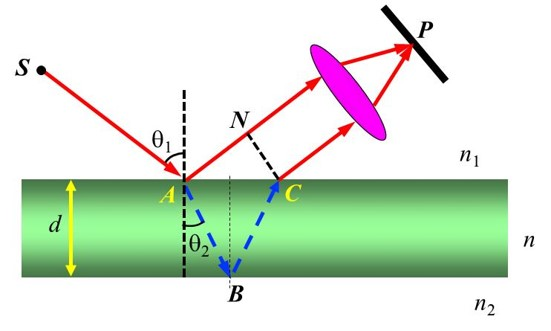
\includegraphics[width=0.4\linewidth]{figures/Equal-inclination}
\end{figure}

\begin{equation*}
  \begin{aligned}
    \Lambda =
  \end{aligned}
  \left\{
    \begin{aligned}
      & 2nk_0 d \cos \theta_2 \pm \pi && \quad\quad n_1 > n_2 < n_3 \ \text{OR} \  n_1 < n_2 > n_3 \\
      & 2nk_0 d \cos \theta_2 && \quad\quad n_1 < n_2 < n_3 \  \text{OR} \  n_1 > n_2 > n_3 \\
    \end{aligned}
  \right.
\end{equation*}

\section{Equal Thickness Interference}

\begin{figure}[H]
  \centering
  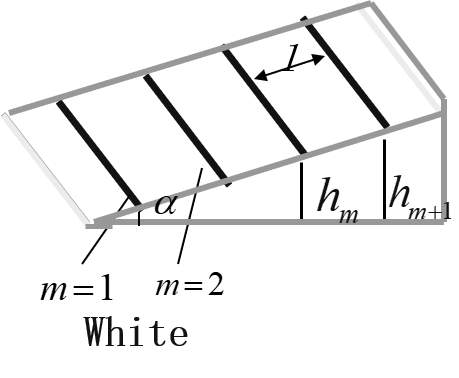
\includegraphics[width=0.4\linewidth]{figures/Equal-thickness}
\end{figure}

\begin{equation*}
  \begin{aligned}
    e = \Delta h = \dfrac{\lambda}{2 n} \quad\quad l = \dfrac{e}{\sin \alpha} = \dfrac{\lambda}{2 n \alpha} \approx \dfrac{\lambda}{2 n \alpha}   
  \end{aligned}
\end{equation*}

\section{Newton's Rings}

\begin{figure}[H]
  \centering
  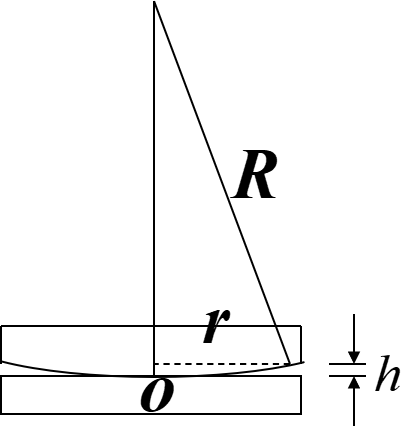
\includegraphics[width=0.4\linewidth]{figures/Newton-Ring}
\end{figure}

\begin{equation*}
  \begin{aligned}
    \Delta = 2 n h + \dfrac{\lambda}{2} = 
  \end{aligned}
  \left\{
    \begin{aligned}
      & k \lambda && \quad\quad \text{White} \\
      & \left( k + \dfrac{1}{2}  \right) \lambda && \quad\quad \text{Black}
    \end{aligned}
  \right.
\end{equation*}

\begin{equation*}
  \begin{aligned}
    h = R - \sqrt{R^2 - r^2} = R \left[ 1 - \sqrt{1 - \left( \dfrac{r}{R}  \right)^2 } \right] \approx \dfrac{r^2}{2R} 
  \end{aligned}
\end{equation*}

\begin{equation*}
  \begin{aligned}
    r^2 = 
  \end{aligned}
  \left\{
    \begin{aligned}
      & \left( k - \dfrac{1}{2}  \right) \dfrac{R \lambda}{n} && \quad\quad \text{White} \\
      & \dfrac{k R \lambda}{n} && \quad\quad \text{Black} 
    \end{aligned}
  \right.
\end{equation*}

%%% Local Variables:
%%% mode: latex
%%% TeX-master: "Optics"
%%% End:
